\FloatBarrier
\section{Behavioral Cloning}
\label{sec::51_bc}
Behavioral cloning in itself is not always related to machine learning but poses one possible way of training a neural network in a supervised manner. The presented concept is easy to understand and got inspired by \cite{bojarski2016end}, where they used it for self-driving cars, and since having a car drive along the road is easier to achieve than having a robot walk around an environment, we will deal with the additional details later to focus on the main points for now. The proposed method utilizes the control loop, which was already introduced in figure \ref{fig::2_cl}. In order to then replace the human user by an artificial agent, we have a human user perform a desired behavior, and copy it. The required extended control loop is shown in figure \ref{fig::222_bc}.
\begin{figure}[h!]
	\centering
	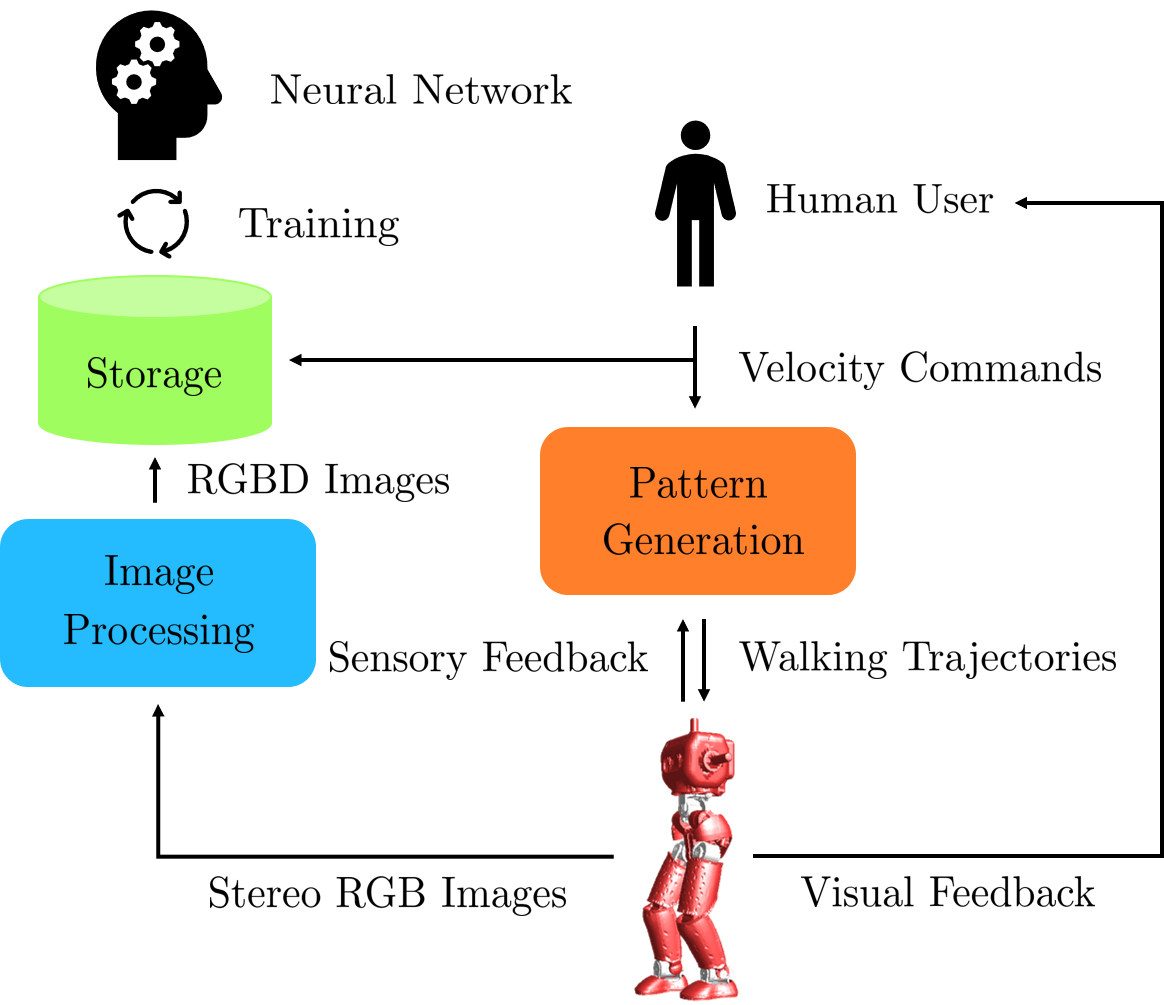
\includegraphics[scale=.5]{chapters/07_autonomous_high_level_control_of_the_walking_pattern_generator/img/behavioral_cloning.png}
	\caption{Pipeline for behavioral cloning. The neural network is trained on stored RGBD images, and corresponding velocity commands that are correlated by a timestamp}
	\label{fig::222_bc}
\end{figure}
It simply takes the velocity commands from the human user and stores it alongside RGBD images with a corresponding timestamp to some storage, where the RGBD images are obtained from stereo RGB images by an image processing step that is explained in section \ref{sec::3_ip}. The timestamp allows to correlate seen images to desired velocities afterward, which in turn enables an artificial agent to train on the stored data. For our purposes, the artificial agent is a neural network. An appropriately chosen network architecture will then enable us to learn the taught behavior and ultimately lets us replace the human user. This procedure relies on prior knowledge to achieve certain tasks, namely the stored data. It is therefore essential to assure that the sampled data, from which we want to learn a task, does not introduce any unwanted bias. That is, we need to take care of the distribution from which we sample in the first place. In principle, it is possible to learn any arbitrary behavior with this technique, but this requires not only good data, but also a vast amount of it. Other algorithms explore the state space on their own, and for which we could, for example, use the taught behavior as prior as well. These algorithms belong to the class of reinforcement learning methods, and we will have a look at a particular one in the next section.
\\\\ TODO
In the previous sections, we have learned about two different approaches to train neural nets on solving certain tasks. Although we came to understand that the complexity of the task to be solved correlates strongly with the amount of data at hand, there exist domains from which it is undeniably easier to do so. To equip a neural network with some prior knowledge by switching the domain may therefore not only be highly desirable but sometimes also needed if the amount or quality of data is not sufficient. One domain which is of special interest when it comes to interacting in a three-dimensional environment is a domain that represents depth information. If there are any, it may sometimes be possible to extract this kind of prior knowledge from a depth camera. As for this work, we need to rely on stereo cameras and powerful algorithms that allow us to compute depth images in real-time. The algorithm that helps us to do so, in terms of the extraction of weighted least squares disparity maps \cite{min2014fast}, will be presented in the following paragraph - Depth Map Extraction.